\documentclass[11pt,a4paper]{article}

\usepackage[margin=2.5cm]{geometry}
\usepackage{amsmath,amssymb,amsthm}
\usepackage{stmaryrd}
\usepackage{graphicx}
\usepackage{tikz}
\usetikzlibrary{positioning,arrows.meta,shapes.geometric,fit,backgrounds}
\usepackage{listings}
\usepackage{xcolor}
\usepackage{booktabs}
\usepackage{hyperref}
\usepackage{cleveref}
\usepackage{enumitem}

\lstdefinestyle{python}{
  language=Python,
  basicstyle=\ttfamily\small,
  keywordstyle=\color{blue!70!black}\bfseries,
  stringstyle=\color{green!40!black},
  commentstyle=\color{gray!80!black}\itshape,
  showstringspaces=false,
  frame=single,
  framesep=2mm,
  xleftmargin=4mm,
  numbers=none,
  breaklines=true,
  columns=fullflexible,
}
\lstdefinestyle{gherkin}{
  basicstyle=\ttfamily\small,
  keywordstyle=\color{purple!70!black}\bfseries,
  morekeywords={Feature,Rule,Scenario,Outline,Examples,Given,When,Then,And},
  frame=single,
  framesep=2mm,
  xleftmargin=4mm,
  numbers=none,
  breaklines=true,
  columns=fullflexible,
}
\lstdefinestyle{coq}{
  language={},
  basicstyle=\ttfamily\small,
  keywordstyle=\color{blue!70!black}\bfseries,
  morekeywords={Definition,Lemma,Proof,Qed,Admitted,Section,End,forall,exists,Fixpoint},
  frame=single,
  framesep=2mm,
  xleftmargin=4mm,
  numbers=none,
  breaklines=true,
  columns=fullflexible,
}

\newtheorem{definition}{Definition}
\newtheorem{example}{Example}
\newtheorem{principle}{Principle}

\title{\textbf{Vericoding: Verification-Driven Development\\
from Behavioural Features to Machine-Checked Proofs}\\[4pt]
\large The \textsf{specsaver} Toolchain}
\author{Gavin Mendel-Gleason\\Scidonia}
\date{July 2026}

\begin{document}
\maketitle

\begin{abstract}
LLM-driven code generation (``vibecoding'') trades correctness for
velocity: generated code may run, but it leaves no durable
specification, no behavioural guarantee, and no machine-checkable
evidence that it satisfies its intended purpose.  We describe a
\emph{vericoding} workflow --- a methodology in which a human-authored
specification is the single source of semantic truth and the primary
lasting artifact, with generated code as a replaceable implementation
detail --- and we present a toolchain, \textsf{specsaver}, to
operationalise it.  The specification takes the form of Gherkin
features (scenario tables), a mathematical contract (pure,
boolean-valued predicates over pre/post-state, frames, and
exceptions), and an abstract state schema; from this single
specification the framework derives executable scenario checks,
fine-grained telemetry assertions, and machine-checked proof
obligations in Rocq (Coq) over a weakest-precondition calculus.
Domain authors declare a \emph{domain} once (DDL, row types, contracts,
features); the framework supplies scenario runners, semantic frame
checking, and differentially-tested stubs for library \emph{theories}
(SQL, logging, OpenTelemetry).  A per-obligation scoreboard of
\textsc{proved}, \textsc{unknown}, and \textsc{disproved} entries
provides a graded feedback cycle from test through proof to
counterexample.  The approach is battle-tested: the core contract
language and theory machinery were extracted from a production
citation-checking platform, and the worked examples include a
production-stolen invitation flow that exercises insertion frames,
multi-table deltas, and time-as-an-argument expiry.
\end{abstract}

%=====================================================================
\section{Introduction}\label{sec:intro}
%=====================================================================

A growing fraction of production code is generated by large language
models.  The resulting programs often ``work'' in the sense that they
execute without crashing, but they leave nothing behind: no
specification of intended behaviour, no evidence of correctness, no
reproducible conformance regime for the next iteration of the
generated code.  We call this pattern \emph{vibecoding}: the developer
prompts, the model emits, the result runs --- and the only long-term
artifact is the code itself, with no human-readable statement of what
the code is supposed to do.

\textbf{Vericoding} inverts this relationship.  In vericoding, the
\emph{specification} is the primary artifact and the code is a
replaceable implementation detail.  The specification is human-written
and human-readable: Gherkin scenarios that domain experts can review,
mathematical contracts that state what must hold before and after each
operation, and framed state declarations that bound exactly what each
operation may read and write.  From this single specification every
downstream verification activity is derived: concrete scenario
execution against real database state, structured telemetry checking,
and machine-checked proof obligations in Rocq (Coq).

\textsf{specsaver} is a toolchain for vericoding.  The core thesis:

\begin{principle}[Single source of semantic truth]
A human-authored specification, written once in the contract
language, is simultaneously: (1) an executable behavioural
specification checked against every row of a Gherkin Examples table,
providing concrete pass/fail feedback in development; (2) a generator
of verification artefacts (witness materialisation, admissibility
checks, frame soundness, derived-state consistency, telemetry
assertions); and (3) the input to a lowering that produces
machine-checked proof obligations about an abstract model of the
implementation --- the ``formalised lockdown'' that sits behind the
runtime checks.
\end{principle}

The pipeline of \cref{fig:pipeline} summarises the development flow:
behavioural intent enters as \emph{features}; features and
implementation are jointly constrained by \emph{contracts}; contracts
drive \emph{testing} against every row of every Examples table; and
finally the same contracts are \emph{lowered} to Rocq and proved ---
the ``formalised lockdown.''

The toolchain supports two development flows.  In
\emph{contract-first} development, features are written first, then
contracts, then an implementation is built against the contract as a
specification, then the implementation is tested and lowered to proof.
In \emph{retrospective} development, a developer begins with existing
feature files and an existing implementation, writes the contract to
capture the behaviour already observed in testing, re-runs the test
suite under contract checking to validate the specification, and then
proceeds to formal proof.  Both flows converge on the same long-lived
artifact --- the contract --- and the same endpoint: a machine-checked
proof that the specification is internally sound.

\begin{figure}[t]
\centering
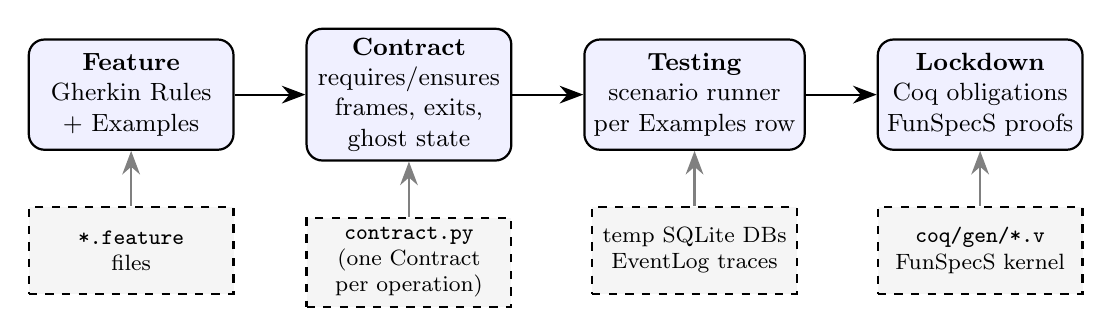
\begin{tikzpicture}[
  stage/.style={draw, rounded corners=2mm, thick, fill=blue!6,
                minimum width=2.6cm, minimum height=1.4cm,
                align=center, font=\small},
  artifact/.style={draw, dashed, thick, fill=gray!8,
                   minimum width=2.6cm, minimum height=1.1cm,
                   align=center, font=\footnotesize},
  arr/.style={-{Stealth[length=3mm]}, thick},
  ]
  \node[stage] (feat) {\textbf{Feature}\\Gherkin Rules\\+ Examples};
  \node[stage, right=0.9cm of feat] (contract) {\textbf{Contract}\\requires/ensures\\frames, exits,\\ghost state};
  \node[stage, right=0.9cm of contract] (test) {\textbf{Testing}\\scenario runner\\per Examples row};
  \node[stage, right=0.9cm of test] (proof) {\textbf{Lockdown}\\Coq obligations\\FunSpecS proofs};

  \node[artifact, below=0.7cm of feat] (fsrc) {\texttt{*.feature}\\files};
  \node[artifact, below=0.7cm of contract] (csrc) {\texttt{contract.py}\\(one Contract\\per operation)};
  \node[artifact, below=0.7cm of test] (tsrc) {temp SQLite DBs\\EventLog traces};
  \node[artifact, below=0.7cm of proof] (psrc) {\texttt{coq/gen/*.v}\\FunSpecS kernel};

  \draw[arr] (feat) -- (contract);
  \draw[arr] (contract) -- (test);
  \draw[arr] (test) -- (proof);
  \draw[arr, gray] (fsrc) -- (feat);
  \draw[arr, gray] (csrc) -- (contract);
  \draw[arr, gray] (tsrc) -- (test);
  \draw[arr, gray] (psrc) -- (proof);
\end{tikzpicture}
\caption{The vericoding pipeline.  Features and contracts are the primary
lasting artifacts; generated code (not shown) is a replaceable
implementation detail.  Every Examples row is exercised against the
contract; the same contract lowers to Coq obligations proved against a
hand-verified kernel.}
\label{fig:pipeline}
\end{figure}

The contributions of this paper are:

\begin{enumerate}[label=(\roman*)]
\item a \emph{contract language} that is the pure, terminating,
  boolean-valued fragment of Python, supporting pre/post-conditions,
  conjunctive exception exits, invariants, derived-state consistency,
  and \emph{semantic frame conditions} (\cref{sec:language});
\item a \emph{symmetric projection architecture} connecting abstract
  specification state to concrete SQLite state through SQLAlchemy, so
  the same snapshot function serves as both pre- and post-state
  (\cref{sec:architecture});
\item a \emph{theory mechanism} that adorns real libraries (SQLAlchemy,
  Python logging, OpenTelemetry) with operational semantics and
  differentially-tested stubs (\cref{sec:theories});
\item a \emph{domain declaration} that collapses per-domain
  infrastructure to a single object (\cref{sec:domains});
\item a \emph{lowering} to Rocq proof obligations over a small
  WP-calculus kernel, with all four example contracts' obligations
  machine-proved; plus a three-way scoreboard of
  \textsc{proved}/\textsc{unknown}/\textsc{disproved} that covers the
  full spectrum from proof to counterexample (\cref{sec:lowering}).
\end{enumerate}

%=====================================================================
\section{Background and Motivation}\label{sec:background}
%=====================================================================

The core failure mode of vibecoding is not that the code is wrong ---
much of it works --- but that the developer loses any ability to
answer ``what is this code supposed to do?'' once the generation
session ends.  The specification is ephemeral (the prompt), the
behavioural checks are absent (no test suite), and the evidence of
correctness is anecdotal (``it worked once'').  When the next LLM
rewrites the function, nothing ties the new version to the old
guarantee.

These faults are more acute in database-backed services, where
silent corruptions --- partial writes across transaction boundaries,
bystander rows mutated outside the declared frame, telemetry that
diverged from committed state --- may be invisible for months and are
costly to prevent by review alone.  The vericoding answer is to leave
the contract in place and treat the code as replaceable: the contract
is checked on concrete data today (so the guarantees are grounded in
executable reality) and lowered to a formal model tomorrow (so the
guarantees acquire mathematical force).

A second motivation is \emph{library semantics}.  Real services call
real libraries --- SQLAlchemy for persistence, Python logging for
telemetry, OpenTelemetry for tracing.  Any verification story that
ignores these calls is a toy.  We therefore need stubs with provable
fidelity: replacements for the real libraries that behave identically
on the fragment the contract language covers, and loudly reject
anything outside it.

%=====================================================================
\section{The Contract Language}\label{sec:language}
%=====================================================================

A \textsf{specsaver} contract is a first-class Python object built by
the \texttt{Contract} constructor (or the \texttt{@contract}
decorator) in what we call the \emph{fluid contract} style
\cite{Meyer92,Leino10}: the contract is a declarative value assembled
from named clauses, not a set of imperative assertions scattered
throughout the code.  \Cref{fig:contract-anatomy} shows its anatomy.

The contract language is the \textbf{pure terminating fragment of
Python}: every clause is a lambda whose body may contain only
arithmetic, comparison, boolean operators, attribute access, and a
small fixed set of combinator calls (\texttt{extends\_by\_one},
\texttt{implies},\linebreak\texttt{safe\_div}).  Side effects, loops,
exceptions, and non-boolean returns are rejected by a static purity
checker before the clause is executed or lowered.  Every clause must
evaluate to a Python \texttt{bool}: contracts reason about truth of
propositions, not about computations.

\begin{definition}[Contract]
A contract for an operation $\mathit{op}$ is a record
$\langle \Sigma, \mathit{args}, \mathsf{pre}, \mathsf{post},
\mathcal{X}, \mathcal{I}, \mathcal{D}, \mathcal{W}, \mathcal{R},
\mathcal{G} \rangle$ where:

\begin{itemize}[nosep,leftmargin=*]
\item $\Sigma$ is the specification state type (observed, derived, ghost components);
\item $\mathit{args}$ is the typed argument record (a frozen dataclass);
\item $\mathsf{pre}(\sigma, a)$ is a boolean predicate on the pre-state and arguments (admissibility);
\item $\mathsf{post}(\sigma, a, r, \sigma')$ is a boolean predicate on pre-state, arguments, result, and post-state (success obligations);
\item $\mathcal{X} = \{\,\langle E_i, C_i, W_i, P_i\rangle \mid i \in [1..n] \,\}$ is the set of exceptional exits, each naming a raised exception type $E_i$, a conjunctive when-condition $C_i$, an exit-specific write frame $W_i$, and exit-specific post-conditions $P_i$;
\item $\mathcal{I}$ is the set of invariants $I(\sigma)$ that must hold in every observable state;
\item $\mathcal{D}$ maps derived field names to pure functions of observed state, checked for consistency at every snapshot;
\item $\mathcal{W}$ and $\mathcal{R}$ are the write and read frame sets: declarative paths into $\Sigma$ that bound what the operation may modify and observe;
\item $\mathcal{G}$ is the ghost-state machinery: a ghost type $G$, an initialisation $\mathsf{init}(w)$ from the scenario witness $w$, a set of ghost transitions $T(\gamma, a, r, \gamma')$, and ghost invariants $I_G(\gamma)$.
\end{itemize}

At the concrete level, each contract clause is a pure, terminating
Python lambda over the fixed argument forms $(\sigma, a)$,
$(\sigma, a, r, \sigma')$, or $(\sigma, a, e)$ (for exception
payloads), statically checked to be boolean-valued and free of side
effects before execution or lowering.\end{definition}

\begin{figure}[t]
\centering
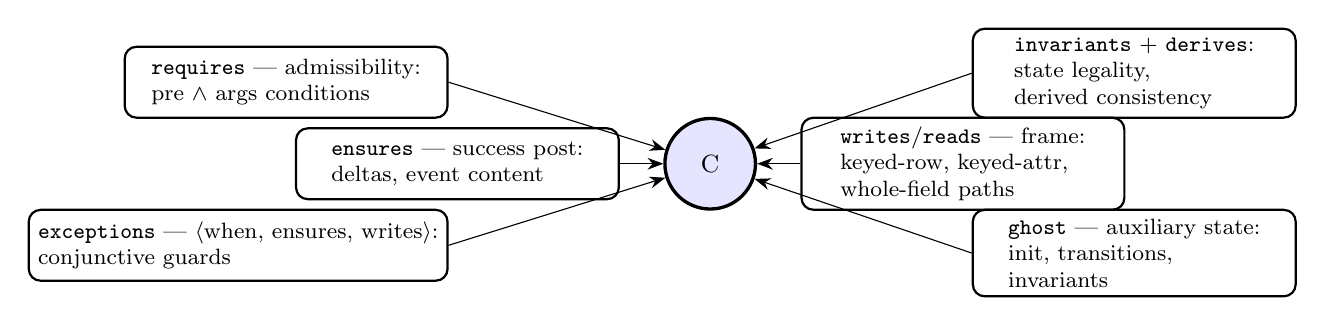
\begin{tikzpicture}[
  clause/.style={draw, thick, rounded corners=1.5mm,
                 minimum width=4.1cm, minimum height=0.9cm,
                 align=left, font=\footnotesize, anchor=west},
  hub/.style={draw, very thick, circle, minimum size=1.15cm,
              fill=blue!10, align=center, font=\small},
  ]
  \node[hub] (c) {C};
  \node[clause, above left=0.15cm and 2.9cm of c] (req)
    {\texttt{requires} — admissibility:\\ pre $\wedge$ args conditions};
  \node[clause, left=0.55cm of c] (ens)
    {\texttt{ensures} — success post:\\ deltas, event content};
  \node[clause, below left=0.15cm and 2.9cm of c] (exc)
    {\texttt{exceptions} — $\langle$when, ensures, writes$\rangle$:\\ conjunctive guards};
  \node[clause, above right=0.15cm and 2.9cm of c] (inv)
    {\texttt{invariants} + \texttt{derives}:\\ state legality,\\derived consistency};
  \node[clause, right=0.55cm of c] (frm)
    {\texttt{writes}/\texttt{reads} — frame:\\ keyed-row, keyed-attr,\\whole-field paths};
  \node[clause, below right=0.15cm and 2.9cm of c] (gh)
    {\texttt{ghost} — auxiliary state:\\ init, transitions,\\invariants};

  \draw[-{Stealth[length=2mm]}] (req.east) -- (c);
  \draw[-{Stealth[length=2mm]}] (ens.east) -- (c);
  \draw[-{Stealth[length=2mm]}] (exc.east) -- (c);
  \draw[-{Stealth[length=2mm]}] (inv.west) -- (c);
  \draw[-{Stealth[length=2mm]}] (frm.west) -- (c);
  \draw[-{Stealth[length=2mm]}] (gh.west) -- (c);
\end{tikzpicture}
\caption{Anatomy of a contract.  Each clause is a pure Python lambda;
all clauses are executable, checkable, and (for the covered fragment)
translatable.}
\label{fig:contract-anatomy}
\end{figure}

\subsection{Semantic frames}

Frame conditions in classical DbC are notoriously verbose: specifying
what \emph{does not} change typically dominates the specification.
\textsf{specsaver} frames are instead \emph{declarative write paths}:

\begin{lstlisting}[style=python]
writes={
    "state.products[sku].reserved",   # one attribute of one keyed row
    "state.invitations[token]",       # whole-row insert of the
                                      # args-resolved key
    "state.reservation_log",          # whole event channel
}
\end{lstlisting}

The checker derives, from these paths alone, the obligation that
everything else is unchanged: every other keyed attribute, every other
keyed row, every other event channel.  A recent refinement admits
\emph{insertion}: keyed-row write paths may \emph{add} the
args-resolved key (e.g.\ a fresh invitation), while deletion is always
rejected.  This is essential for operations such as \texttt{invite}
that create rows.

\subsection{Exceptional exits}

Exceptions are specified as data, not control flow:

\begin{lstlisting}[style=python]
exceptions=[
    ExcExit(
        raises=InsufficientStockError,
        when=[lambda state, args:
                  state.observed.products[args.sku].on_hand
                - state.observed.products[args.sku].reserved
                < args.quantity],
        writes={"state.failure_log"},
        ensures=[lambda state, args, exc, after_s: extends_by_one(
            state.observed.failure_log,
            after_s.observed.failure_log,
            lambda f: f.sku == args.sku
                      and f.available == exc.available
                      and f.reason == InsufficientStockError.code)],
    )]
\end{lstlisting}

The runner checks that when the \texttt{when} clauses hold, the
exception raised is the declared one, that the failure telemetry
contains exactly one new event with the exact declared fields, and
that nothing outside the exit's writes changed.  The classical
``exceptions leave state untouched'' discipline falls out of the
default empty frame.

\subsection{Ghost state}

Ghost state is auxiliary specification state invisible to the
implementation --- e.g.\ the total stock present before the scenario,
used to state conservation laws that are not expressible over the
concrete DB alone.  Ghost state is initialised from the scenario
witness, constrained by transition relations per call, and held to
global ghost invariants.

%=====================================================================
\section{Symmetric Projection Architecture}\label{sec:architecture}
%=====================================================================

The central architectural problem is the bridge between the abstract
specification state (a frozen dataclass of observed, derived, and
ghost components) and the concrete execution world (a live SQLite
database plus a telemetry log).  \textsf{specsaver}'s answer is
\emph{symmetry}: one function, used twice.

\begin{figure}[t]
\centering
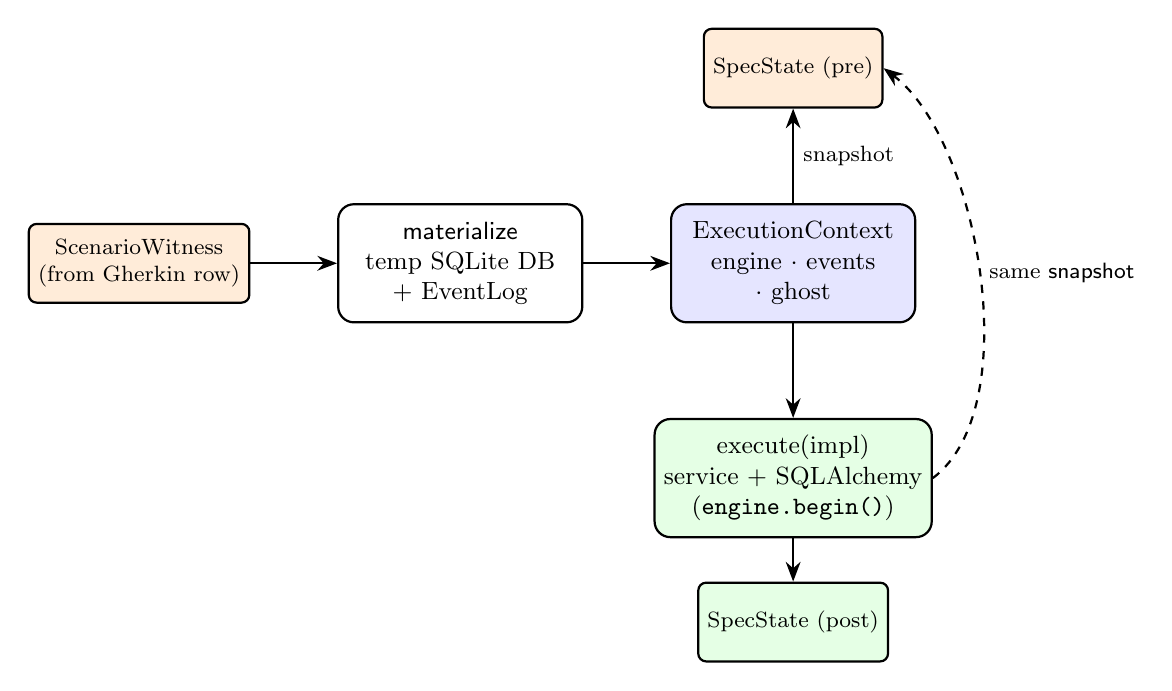
\begin{tikzpicture}[
  box/.style={draw, thick, rounded corners=2mm, minimum width=3.1cm,
              minimum height=1.5cm, align=center, font=\small},
  small/.style={draw, thick, fill=orange!15, rounded corners=1mm,
                minimum width=2.2cm, minimum height=1.0cm,
                align=center, font=\footnotesize},
  arr/.style={-{Stealth[length=2.5mm]}, thick},
  ]
  \node[small] (wit) {ScenarioWitness\\(from Gherkin row)};
  \node[box, right=1.1cm of wit] (mat) {\textsf{materialize}\\temp SQLite DB\\+ EventLog};
  \node[box, right=1.1cm of mat, fill=blue!10] (ctx) {ExecutionContext\\engine $\cdot$ events\\$\cdot$ ghost};
  \node[box, below=1.2cm of ctx, fill=green!10] (impl) {execute(impl)\\service + SQLAlchemy\\(\texttt{engine.begin()})};
  \node[small, above=1.2cm of ctx] (pre) {SpecState (pre)};
  \node[small, below=0.55cm of impl, fill=green!10] (post) {SpecState (post)};

  \draw[arr] (wit) -- (mat);
  \draw[arr] (mat) -- (ctx);
  \draw[arr] (ctx) -- node[right, font=\footnotesize]{snapshot} (pre);
  \draw[arr] (ctx) -- (impl);
  \draw[arr] (impl) -- (post);
  \draw[arr, dashed] (impl.east) .. controls +(1.2,0.9) and +(1.2,-0.9)
        .. node[right, font=\footnotesize]{same \textsf{snapshot}} (pre.east);
\end{tikzpicture}
\caption{The symmetric projection.  \textsf{snapshot(context)} projects
the concrete world into the abstract SpecState both before and after
execution; contracts compare pre and post.  The service talks only to
SQLAlchemy; the same service code runs on a real SQLite file and on the
theory stub (\cref{sec:theories}).}
\label{fig:symmetry}
\end{figure}

\begin{definition}[Symmetry requirement]
Let $\mathsf{snap}: \mathit{Ctx} \to \mathit{SpecState}$ be the
projection.  For every scenario, the runner evaluates all contract
clauses against $\mathit{pre} = \mathsf{snap}(c)$ and
$\mathit{post} = \mathsf{snap}(\mathit{impl}(c))$, for the same
$\mathsf{snap}$.  There is no separate ``read'' and ``check'' path.
\end{definition}

The scenario runner then performs, per Examples row:

\begin{enumerate}[label=\arabic*.]
\item \textbf{materialize} the witness into a context (temp SQLite file);
\item \textbf{pre-check}: invariants on the pre-state, then
  admissibility (\texttt{requires}) --- \texttt{rejected} outcomes are
  expected to fail admissibility, \texttt{error:...} outcomes to pass it;
\item \textbf{execute} the effect-emitting wrapper around the service;
\item \textbf{frame check}: everything outside the declared writes
  unchanged (for success) or the exit's writes (for exceptions);
\item \textbf{derived check}: derived fields recomputed equal their
  \texttt{derives} definitions;
\item \textbf{post-check}: \texttt{ensures} or the matching
  \texttt{ExcExit.ensures}; invariants on the post-state.
\end{enumerate}

Crucially, the service is ordinary production code: SQLAlchemy
\texttt{engine.begin()} transactions, \texttt{text()} statements,
domain exceptions.  Nothing in it knows about contracts, snapshots, or
scenario rows.

%=====================================================================
\section{Examples with Databases}\label{sec:examples}
%=====================================================================

We present three domains of increasing structural interest, all
against SQLite through SQLAlchemy.

\subsection{Inventory: deltas and conditional telemetry}

The inventory domain models stock reservations over a single
\texttt{products} table.  The reserve contract's essential clauses,
written in the mathematical style they realise:

\[
\mathsf{pre}(s, a) \;=\; a.\mathit{quantity} > 0 \;\wedge\; a.\mathit{sku} \in s.\mathit{products}
\]

\[
\mathsf{post}(s, a, r, s') \;=\;
\begin{array}[t]{l}
s'.\mathit{products}[a.\mathit{sku}].\mathit{reserved}
  \;=\; s.\mathit{products}[a.\mathit{sku}].\mathit{reserved} + a.\mathit{quantity} \\[2pt]
{}\wedge\; \mathsf{extends\_by\_one}(s.\mathit{reservation\_log},\, s'.\mathit{reservation\_log},\,
      \lambda e.\; e.\mathit{sku} = a.\mathit{sku}) \\[2pt]
{}\wedge\; \mathsf{implies}(\mathit{crossed}(s,a,s'),\;
      \mathsf{extends\_by\_one}(s.\mathit{alert\_log},\, s'.\mathit{alert\_log},\,
        \lambda a.\; a.\mathit{sku} = a.\mathit{sku}))
\end{array}
\]

\[
\mathcal{X} = \bigl\{\,
\langle \mathsf{InsufficientStock},\; s.\mathit{available}(a.\mathit{sku}) < a.\mathit{quantity},\;
       \{\mathit{failure\_log}\},\; \mathsf{failure\_ensures} \rangle \,\bigr\}
\]

with $\mathcal{W} = \{\,\mathit{products}[sku].\mathit{reserved},\; \mathit{reservation\_log},\; \mathit{gauge\_log},\; \mathit{alert\_log}\,\}$.
The frame checker derives, from $\mathcal{W}$ alone, that every other
state path is unchanged: on-hand, reorder point, all other product
rows, and the release/restock/failure channels.  The invariant
$\forall p \in \mathit{products}.\; 0 \leq p.\mathit{reserved} \leq
p.\mathit{on\_hand}$ is checked in both pre- and post-state.

The Gherkin source rows are ordinary scenario outlines; the domain
declares a witness builder mapping each row into an initial
\texttt{products} dict and a typed \texttt{ReserveArgs}.

\subsection{Bank transfer: multi-key deltas and invariants}

The transfer contract moves funds between two rows of one table, with
a balance-nonnegativity invariant and currency-mismatch and
insufficient-funds exits.  Its writes are two keyed attributes on
\emph{different} keys --- demonstrating that frames compose over
multi-delta operations --- and its ensures include a conservation law
(total balance preserved) and a negative-balance legality post-state
invariant.  The obligation generator lowers this to a two-key nested
insert with conjunctive exception arms; all 7 obligations prove.

\subsection{Invitations: insertion, multi-table state, and time}

The invitations domain, stolen from a production service
(\textsf{paperchecker}), exercises the newest machinery:

\[
\mathsf{post}_{\mathit{invite}}(s, a, r, s') \;=\;
\begin{array}[t]{l}
s'.\mathit{invitations}[a.\mathit{token}].\mathit{status} = \text{``pending''} \\[1pt]
{}\wedge\; s'.\mathit{invitations}[a.\mathit{token}].\mathit{expires\_at}
       \;=\; a.\mathit{now} + 7\!\cdot\!86400 \\[1pt]
{}\wedge\; \mathsf{extends\_by\_one}(s.\mathit{invite\_log},\, s'.\mathit{invite\_log},\,
      \lambda e.\; e.\mathit{invitee\_email} = a.\mathit{invitee\_email})
\end{array}
\]

with $\mathcal{W}_{\mathit{invite}} = \{\,\mathit{invitations}[token],\; \mathit{invite\_log}\,\}$

\[
\mathcal{X}_{\mathit{accept}} = \bigl\{\,
\langle \mathsf{InvitationExpired},\;
       \mathit{pending}(s,a) \wedge a.\mathit{now} > s.\mathit{invitations}[a.\mathit{token}].\mathit{expires\_at},\;
       \{\mathit{accept\_failure\_log}\},\; \ldots \rangle \,\bigr\}
\]

\[
\mathsf{post}_{\mathit{accept}}(s, a, r, s') \;=\;
\begin{array}[t]{l}
s'.\mathit{invitations}[a.\mathit{token}].\mathit{status} = \text{``accepted''} \\[1pt]
{}\wedge\; s'.\mathit{members}[a.\mathit{user\_id}].\mathit{org\_id}
       \;=\; s.\mathit{invitations}[a.\mathit{token}].\mathit{org\_id} \\[1pt]
{}\wedge\; s'.\mathit{members}[a.\mathit{user\_id}].\mathit{role}
       \;=\; s.\mathit{invitations}[a.\mathit{token}].\mathit{role} \\[1pt]
{}\wedge\; s'.\mathit{users}[a.\mathit{user\_id}].\mathit{default\_org}
       \;=\; s.\mathit{invitations}[a.\mathit{token}].\mathit{org\_id} \\[1pt]
{}\wedge\; \mathsf{extends\_by\_one}(s.\mathit{accept\_log},\, s'.\mathit{accept\_log},\,
      \lambda e.\; e.\mathit{user\_id} = a.\mathit{user\_id})
\end{array}
\]

with $\mathcal{W}_{\mathit{accept}} = \{\,\mathit{invitations}[token].\mathit{status},\;
       \mathit{members}[user\_id],\; \mathit{users}[user\_id].\mathit{default\_org},\;
       \mathit{accept\_log}\,\}$.

Two design decisions make this contract-first: the accept-link token
is a caller-supplied argument (so the insert key is args-resolved and
the frame can see it), and \texttt{now} is an integer epoch argument
(so expiry is a pure comparison, translatable and deterministic).
Accepting touches three tables; the frame still derives that the
fourth logical region --- the email channel, user emails, every other
invitation --- is untouched.

\begin{table}[t]
\centering
\small
\begin{tabular}{@{}lcccc@{}}
\toprule
Domain & Tables & Operations & Feature rows & Frame shape \\
\midrule
inventory & 1 & reserve, release, restock & 22 & keyed-attr deltas \\
bank\_transfer & 2 & transfer & 11 & multi-key deltas \\
invitations & 3 & invite, accept & 9 & insert + multi-table \\
\bottomrule
\end{tabular}
\caption{The three database-backed example domains.  All feature rows
are executed and checked by the generic conformance suite.}
\label{tab:domains}
\end{table}

%=====================================================================
\section{Theories: Adorning Libraries with Semantics}\label{sec:theories}
%=====================================================================

Verification of library-calling code requires a stance on what the
library does.  \textsf{specsaver}'s stance is the \emph{theory}: a
first-order operational model of the library's covered fragment,
paired with a stub that behaves identically to the real library on
that fragment --- and rejects everything else loudly.

\begin{figure}[t]
\centering
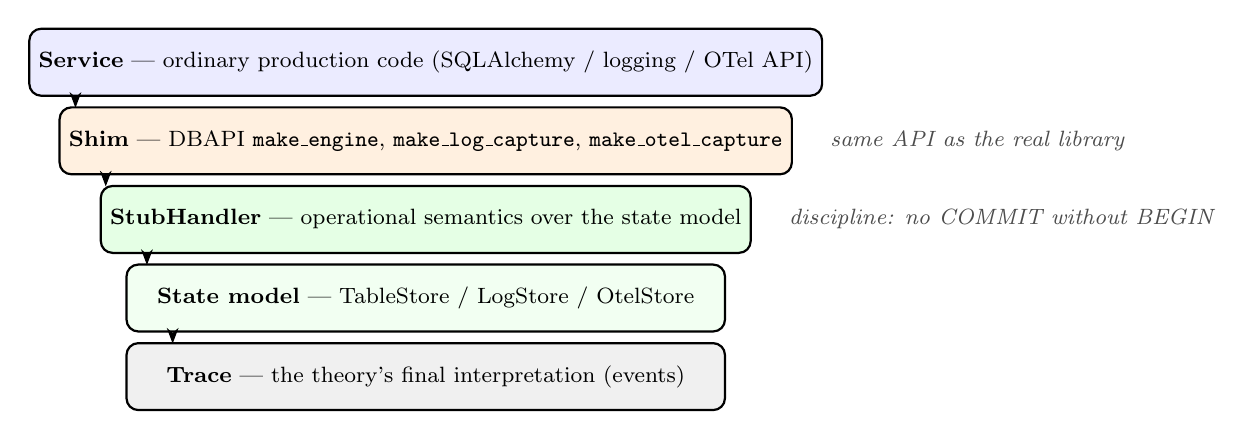
\begin{tikzpicture}[
  layer/.style={draw, thick, rounded corners=1.5mm,
                minimum width=7.6cm, minimum height=0.85cm,
                align=left, font=\footnotesize, anchor=west},
  note/.style={font=\footnotesize\itshape, text=gray!60!black},
  ]
  \node[layer, fill=blue!8] (service) {\textbf{Service} — ordinary
    production code (SQLAlchemy / logging / OTel API)};
  \node[layer, below=0.12cm of service, fill=orange!12] (shim)
    {\textbf{Shim} — DBAPI \texttt{make\_engine},
     \texttt{make\_log\_capture}, \texttt{make\_otel\_capture}};
  \node[layer, below=0.12cm of shim, fill=green!10] (handler)
    {\textbf{StubHandler} — operational semantics over the state model};
  \node[layer, below=0.12cm of handler, fill=green!5] (model)
    {\textbf{State model} — TableStore / LogStore / OtelStore};
  \node[layer, below=0.12cm of model, fill=gray!12] (trace)
    {\textbf{Trace} — the theory's final interpretation (events)};

  \node[note, right=0.35cm of shim] {same API as the real library};
  \node[note, right=0.35cm of handler] {discipline: no COMMIT without BEGIN};

  \draw[-{Stealth[length=2mm]}] (service.south west) ++(0.6,0) -- ++(0,-0.14);
  \draw[-{Stealth[length=2mm]}] (shim.south west) ++(0.6,0) -- ++(0,-0.14);
  \draw[-{Stealth[length=2mm]}] (handler.south west) ++(0.6,0) -- ++(0,-0.14);
  \draw[-{Stealth[length=2mm]}] (model.south west) ++(0.6,0) -- ++(0,-0.14);
\end{tikzpicture}
\caption{The theory stack.  The service is written once, against the
real library API; the shim connects that API to the stub; the stub
interprets actions over a pure state model and records the trace.
Differential tests run the same programs against stub and real
library and require identical observable behaviour.}
\label{fig:theory-stack}
\end{figure}

\subsection{The SQL theory}

The SQL theory covers a deliberately small fragment: equality-\textsc{where}
\texttt{SELECT} (with optional \texttt{ORDER BY} ascending), single-row
\texttt{INSERT}, and \texttt{UPDATE} with \texttt{SET col = col $\pm$
expr}.  Statements are parsed by \texttt{sqlglot} into an action model;
anything outside the fragment raises \texttt{UnsupportedStatementError}.

The stub handler interprets the action model over an immutable
\texttt{TableStore}, records the trace (\texttt{Begin}, \texttt{Execute},
\texttt{FetchOne}, \texttt{Commit}, \texttt{Rollback}), and enforces
transaction discipline.  Crucially, the same handler is exposed
through a PEP-249 DBAPI shim, so \emph{unmodified SQLAlchemy service
code runs on the theory}.  The sqlite dialect's deferred-autobegin
semantics is modelled at the connection level; \texttt{commit()} and
\texttt{rollback()} are, as in real sqlite3, no-ops without an open
transaction, while the SQL-string path keeps strict discipline.

Fidelity is established differentially: a battery of programs
(SELECT/UPDATE/INSERT/BEGIN/COMMIT/ROLLBACK sequences) run both
against real in-memory SQLite and against SQLAlchemy-over-stub, and
fetches, final table contents, error classes, and traces must agree.

\subsection{Logging and OpenTelemetry theories}

The same six-layer shape repeats.  For \textbf{logging}, the action
model is a \texttt{LogEmit} (level, logger name, message, extra dict);
the stub is a \texttt{logging.Handler} subclass; the capture context
manager installs it at DEBUG level and restores state on exit; the
store offers \texttt{by\_level}/\texttt{by\_logger} facet views.
Differential fidelity compares against a real \texttt{StreamHandler}.

For \textbf{OpenTelemetry}, the action model is a \texttt{SpanRecord}
(name, ids, attributes, events, status, timestamps); the stub is an
\texttt{opentelemetry.sdk.trace.SpanProcessor}; the capture context
manager builds a fresh \texttt{TracerProvider} with the stub attached
(resetting OTel's one-set guard so sequential captures in a test
process work).  Differential fidelity compares against
\texttt{InMemorySpanExporter}.

\begin{principle}[Theory conformance]
A theory is admissible only if: (1) its stub and the real library
agree observationally on a differential suite; (2) its translator
rejects out-of-fragment input loudly, never silently; (3) its state
model and trace are pure data.  New theories (e.g.\ an HTTP client, a
queue) follow the same checklist.
\end{principle}

%=====================================================================
\section{Domains: Declaring a Verification Unit Once}\label{sec:domains}
%=====================================================================

Experience with three domains revealed a stable shape: only
types, service, contract, features, and witness builders are genuinely
domain content; everything else (event log, temp-DB lifecycle,
projection mechanics, runner wiring, test dispatch) was byte-identical
infrastructure copied per domain.  The \texttt{SqlDomain} declaration
(\cref{fig:domain-decl}) collapses the latter.

\begin{figure}[t]
\centering
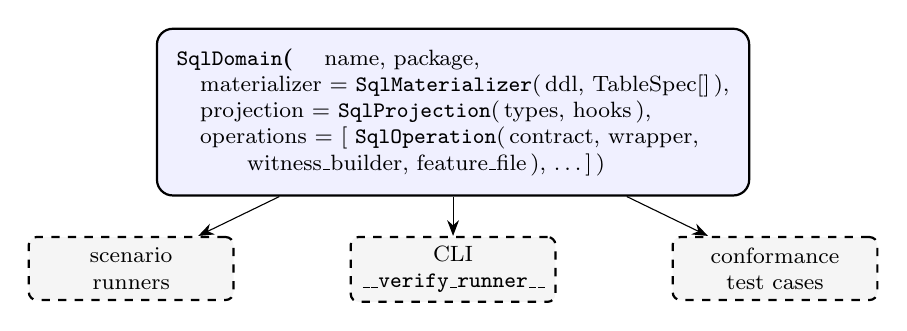
\begin{tikzpicture}[
  decl/.style={draw, thick, fill=blue!6, rounded corners=2mm,
               minimum width=6.6cm, align=left, font=\footnotesize,
               inner sep=2.5mm},
  gen/.style={draw, dashed, thick, fill=gray!8, rounded corners=1mm,
              minimum width=2.6cm, minimum height=0.8cm,
              align=center, font=\footnotesize},
  ]
  \node[decl] (d) {\textbf{\texttt{SqlDomain}(}
    \quad name, package,\\
    \quad materializer = \texttt{SqlMaterializer}(\,ddl, TableSpec[]\,),\\
    \quad projection = \texttt{SqlProjection}(\,types, hooks\,),\\
    \quad operations = [ \texttt{SqlOperation}(\,contract, wrapper,\\
    \quad\qquad witness\_builder, feature\_file\,), \ldots ]\,)};
  \node[gen, below left=0.5cm and -1.0cm of d] (r1) {scenario\\runners};
  \node[gen, below=0.5cm of d] (r2) {CLI\\\texttt{\_\_verify\_runner\_\_}};
  \node[gen, below right=0.5cm and -1.0cm of d] (r3) {conformance\\test cases};
  \draw[-{Stealth[length=2mm]}] (d) -- (r1);
  \draw[-{Stealth[length=2mm]}] (d) -- (r2);
  \draw[-{Stealth[length=2mm]}] (d) -- (r3);
\end{tikzpicture}
\caption{One \texttt{SqlDomain} declaration derives runners, CLI
dispatch, and the conformance suite.  The contract's \texttt{observe}
is wired to the shared projection automatically (breaking the
contract--projection import cycle).}
\label{fig:domain-decl}
\end{figure}

A \texttt{TableSpec} names a table's columns, primary key, and the
witness attribute carrying its initial rows; from these the
materializer generates DDL execution, \texttt{DELETE}+
\texttt{INSERT} seeding, engine construction, and teardown.  The
projection queries each declared table and passes row dicts plus the
event log to two small domain hooks (\texttt{extract\_observed},
\texttt{compute\_derived}).  Domains with irregular tables (the
key/value \texttt{limits} table in bank transfer) declare a
\texttt{populate\_extra} hook and query such tables manually inside
\texttt{extract\_observed}.

The conformance suite iterates every registered domain, every
operation, and every Examples row, running the full check pipeline of
\cref{sec:architecture}.  Adding a domain is now: types, service,
contracts, features, witness builders, one declaration --- with the
conformance guarantee that malformed pieces fail loudly at import
time rather than silently at scenario time.

%=====================================================================
\section{Lowering to Proof Obligations}\label{sec:lowering}
%=====================================================================

The final stage is the ``formalised lockdown'': the same contract is
introspected and emitted as a Rocq file of proof obligations over a
small, hand-verified kernel.

\subsection{The kernel}

The Coq side comprises three layers.  \textbf{SnakeletExn} is a tiny
imperative language with dictionaries, lists, exceptions, and an
evaluation relation.  A \textbf{weakest-precondition calculus} over it
(SnakeletExnWp) provides the standard structural tactics.
\textbf{FunSpecS} is a specification kernel: a function table maps
operation names to stateful specs $(\mathit{pre}, \mathit{post})$
where \emph{post} constrains the result and the list of heap-cell
updates; a library of proven support lemmas (dictionary lookup/insert,
store invariants) lives in \texttt{SpecPrelude}.

\subsection{The generator}

\texttt{specsaver.lower} introspects a \texttt{Contract} into a
\emph{shape}: typed row fields, per-key deltas, scalar preconditions,
conjunctive exception arms, and the invariant's comparison structure.
Anything outside the supported shape raises
\texttt{UnsupportedShapeError} rather than emitting a wrong proof.
The emitter then produces a file containing, per operation:
\texttt{gen\_pre}/\texttt{gen\_post} (and per-arm exception
pre/post), a function table, totality lemmas, invariant-preservation
lemmas, and the obligation set --- admissibility sanity, spec
consistency, per-exit consistency, exit coverage, invariant
preservation, and frame soundness (\cref{fig:lowering}).

\begin{figure}[t]
\centering
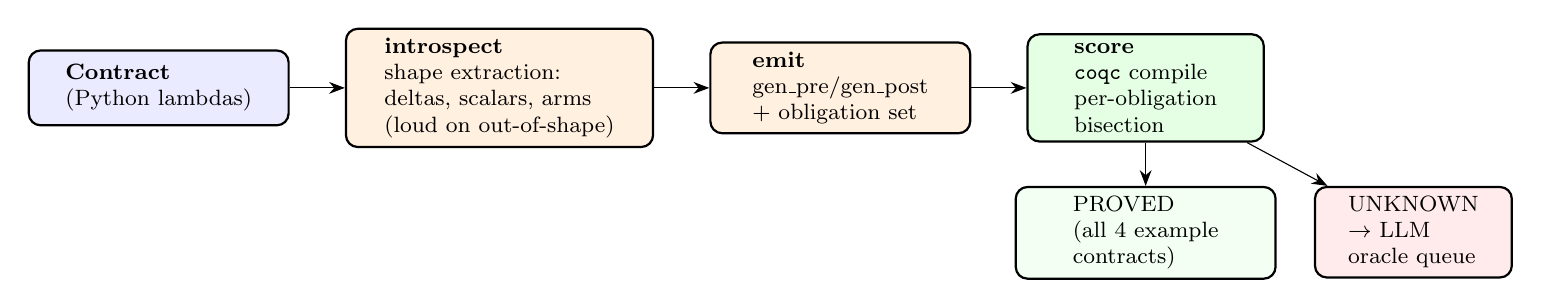
\begin{tikzpicture}[
  node/.style={draw, thick, rounded corners=1.5mm, minimum height=0.95cm,
               align=left, font=\footnotesize, anchor=west},
  ]
  \node[node, fill=blue!8, minimum width=3.3cm] (c) {\textbf{Contract}\\(Python lambdas)};
  \node[node, fill=orange!12, minimum width=3.9cm, right=0.7cm of c]
        (i) {\textbf{introspect}\\shape extraction:\\deltas, scalars, arms\\(loud on out-of-shape)};
  \node[node, fill=orange!12, minimum width=3.3cm, right=0.7cm of i]
        (e) {\textbf{emit}\\gen\_pre/gen\_post\\+ obligation set};
  \node[node, fill=green!10, minimum width=3.0cm, right=0.7cm of e]
        (s) {\textbf{score}\\\texttt{coqc} compile\\per-obligation\\bisection};

  \node[node, fill=green!5, minimum width=3.3cm, below=0.55cm of s]
        (ok) {PROVED\\(all 4 example\\contracts)};
  \node[node, fill=red!8, minimum width=2.5cm, below=0.55cm of s, xshift=3.4cm]
        (unk) {UNKNOWN\\$\to$ LLM\\oracle queue};

  \draw[-{Stealth[length=2mm]}] (c) -- (i);
  \draw[-{Stealth[length=2mm]}] (i) -- (e);
  \draw[-{Stealth[length=2mm]}] (e) -- (s);
  \draw[-{Stealth[length=2mm]}] (s) -- (ok);
  \draw[-{Stealth[length=2mm]}] (s) -- (unk);
\end{tikzpicture}
\caption{The lowering pipeline.  The harness compiles whole-file, then
bisects per obligation on failure, yielding a PROVED/UNKNOWN
scoreboard; UNKNOWNs are packaged as self-contained proof problems for
the oracle queue.}
\label{fig:lowering}
\end{figure}

An example fragment of generated code for reserve:

\begin{lstlisting}[style=coq]
Definition gen_post (sigma : sn_state) (vs : list sn_val)
    (r : Result) (ups : cell_updates) : Prop :=
  exists sku order quantity store_d on_hand_sku reserved_sku
         reorder_point_sku,
    vs = [LitString sku; LitString order; LitInt quantity] /\
    sigma !! store_loc = Some (LitDict store_d) /\
    dict_lookup_str sku store_d =
      Some (row_of on_hand_sku reserved_sku reorder_point_sku) /\
    r = RVal (LitInt reserved_sku) /\
    ups = [(store_loc, LitDict (dict_insert_str sku
            (row_of on_hand_sku (reserved_sku + quantity)
                    reorder_point_sku) store_d))].
\end{lstlisting}

All four example contracts currently generate \emph{and prove}: reserve
(6/6 obligations), release (6/6), restock (4/4), transfer (7/7),
including frame soundness and invariant preservation.  Trace-cell
obligations (list-append post-states for event channels) are the
active development front (\cref{sec:related}).

The per-obligation scoreboard distinguishes three statuses.
\textsc{proved} is the final word: the machine has checked the
obligation against the kernel and closed it.  \textsc{unknown} means
the obligation did not close within the proof heuristics; it is
queued for the LLM-based oracle.  \textsc{disproved} is a third
status not yet wired into the harness but natural in our setting: the
scenario runner already exercises every contract clause against
concrete data from the Gherkin tables, and a failing runtime check for
a well-formed contract is a counterexample --- concrete evidence that
the specification is inconsistent.  Surfacing this as a first-class
scoreboard entry closes the loop: proofs tell you what must be true;
counterexamples tell you what cannot be true.



%=====================================================================
\section{Related and Future Work}\label{sec:related}
%=====================================================================

\textbf{Design by Contract} (Eiffel and successors) provides runtime
assertions without a path to mechanised proof; \textsf{specsaver}
keeps the executable-contract ergonomics and adds the lowering.
\textbf{Property-based testing} (Hypothesis, QuickCheck) generates
data but keeps properties informal; our contracts are simultaneously
test oracles and proof obligations.  \textbf{KeY, Frama-C, and Dafny}
verify source-level contracts but require the source language to be
the specification language; we instead verify an abstract model
aligned with the contract's declared frame, keeping production code
unmodified.  \textbf{Separation-logic-based verification of
library-calling code} typically models libraries by axiomatisation;
our theories are \emph{tested} against the real libraries, replacing
axioms by evidence.

Current work: (i) trace-cell obligations in the lowering --- event
channels as list cells with \texttt{extends\_by\_one} as list-append
post-conditions (the runtime side already enforces these); (ii)
incremental re-verification keyed on contract/body hashes;
(iii) loop and sequence support in the obligation generator;
(iv) surfacing \textsc{disproved} counterexamples from the runner
into the scoreboard.

%=====================================================================
\section{Conclusion}\label{sec:conclusion}
%=====================================================================

A vericoding workflow offers a concrete alternative to the vibecoding status quo.  Where
vibecoding leaves code and hope, vericoding leaves a specification and
evidence: human-readable contracts that domain experts can review,
concrete scenario checks that catch regressions before deployment, and
machine-checked proofs that establish universal properties about the
abstract model.  The generated code is free to change --- move from
raw sqlite3 to SQLAlchemy, add a caching layer, replay events into a
different schema --- so long as it continues to satisfy the same
contract.  The specification survives.

Three ingredients make this practical: the symmetric projection that
grounds contracts in real database state; the theory mechanism that
replaces axiomatic library models with differentially-tested stubs;
and the domain declaration that reduces a new verification unit to its
irreducible content.  The examples --- reservation, transfer, and a
production-stolen invitation flow from a real citation-checking
platform --- show that the idiom scales to multi-table, multi-exit,
insert-bearing systems.  The
\textsc{proved}/\textsc{unknown}/\textsc{disproved} scoreboard
completes the feedback cycle: every row of every feature is a test;
every contract is a proof obligation; and every runtime failure of a
well-formed contract is a counterexample ready to be surfaced.



%=====================================================================
\begin{thebibliography}{10}

\bibitem{Meyer92}
Bertrand Meyer.
\textit{Applying ``Design by Contract''}.
IEEE Computer, 25(10):40--51, 1992.

\bibitem{Leino10}
K.\ Rustan M.\ Leino and Peter M\"uller.
\textit{Using the Spec\# Language, Methodology, and Tools to Write
Bug-Free Programs}.
In LASER Summer School 2008/2009, LNCS 6029, Springer, 2010.

\bibitem{SpecSaver25}
Gavin Mendel-Gleason.
\textit{specsaver: Specification-Driven Verification}.
Source code and documentation. \texttt{https://github.com/scidonia/specsaver}, 2025--2026.

\bibitem{Gherkin}
Cucumber Ltd.
\textit{Gherkin Reference}.
\texttt{https://cucumber.io/docs/gherkin/reference/}, 2025.

\bibitem{QuickCheck}
Koen Claessen and John Hughes.
\textit{QuickCheck: A Lightweight Tool for Random Testing of Haskell Programs}.
In ICFP 2000.

\bibitem{SepLogic}
John C.\ Reynolds.
\textit{Separation Logic: A Logic for Shared Mutable Data Structures}.
In LICS 2002.

\bibitem{FunSpecS}
Scidonia.
\textit{SnakeletExn and FunSpecS: A Small Imperative Language and
Weakest-Precondition Specification Kernel}.
Coq development, 2026.

\end{thebibliography}

\end{document}
